
\section{Cave Discoveries}

Our major cave finds this year are described as these separate
developments within \passage[mountain]{Tolminski Migovec}:


\subsection{Winter Action}

In October 2011, a joint effort by ICCC and JSPDT was made to forge the
connection. While the connection was ultimately unsuccessful, important
survey work of recent years' efforts in \passage{Kavkna Jama} clearly
showed which part of \passage{M2} was closest to \passage{Vrtnarija}. As a
result, the focus of exploration shifted from the bottom of \passage{M2} to
\passage{Wizard of Oz}, a bolt climb at -350 m that was pushed in 2009 (and surveyed in 2011).


\begin{marginfigure}
\checkoddpage \ifoddpage \forcerectofloat \else \forceversofloat \fi
\centering
 \frame{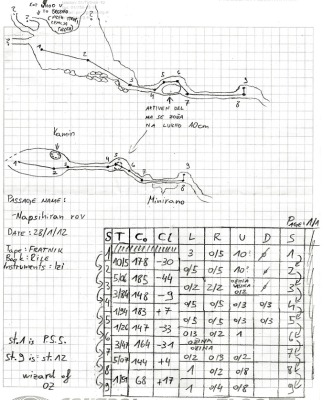
\includegraphics[width=\linewidth]{2012/discoveries/m2_napsihiran_rov-png-scaled.jpg}} 
 \caption{Survey measurements from \passage{M2}.}
 \label{m2 napshiran rov survey}
\end{marginfigure}

In the months between the October 2011 weekend and the start of the 2012 Sledi
Vetra expedition, the JSPDT had multiple pushing trips at \passage{Wizard
of Oz}. The silted rift was dug through and widened to gain a fairly
large, clean chamber with no obvious way on. A small passage about 3 m
from the floor was expanded into yet more narrow and muddy crawls,
eventually ending in a smaller chamber. Once again, easy progress was
hampered by an extremely tight crawl.


\subsection{\passage{Vrtnarija} / \passage{M2} (\passage{Kavkna Jama})}

Three `connection' trips were carried out during the expedition. On the
first two attempts, simultaneous trips were run to \passage{Captain Kangaroo} in
\passage{Vrtnarija} and \passage{Wizard of Oz} in \passage{M2}. Unfortunately,
progress past the tight crawl in \passage{Wizard of Oz} proved elusive as
expanding it was slow work. However, on both occasions teams in
\passage{Vrtnarija} were able to hear the sounds of the \passage{M2} team
drilling and hammering.

\begin{marginfigure}
\checkoddpage \ifoddpage \forcerectofloat \else \forceversofloat \fi
\centering
 \frame{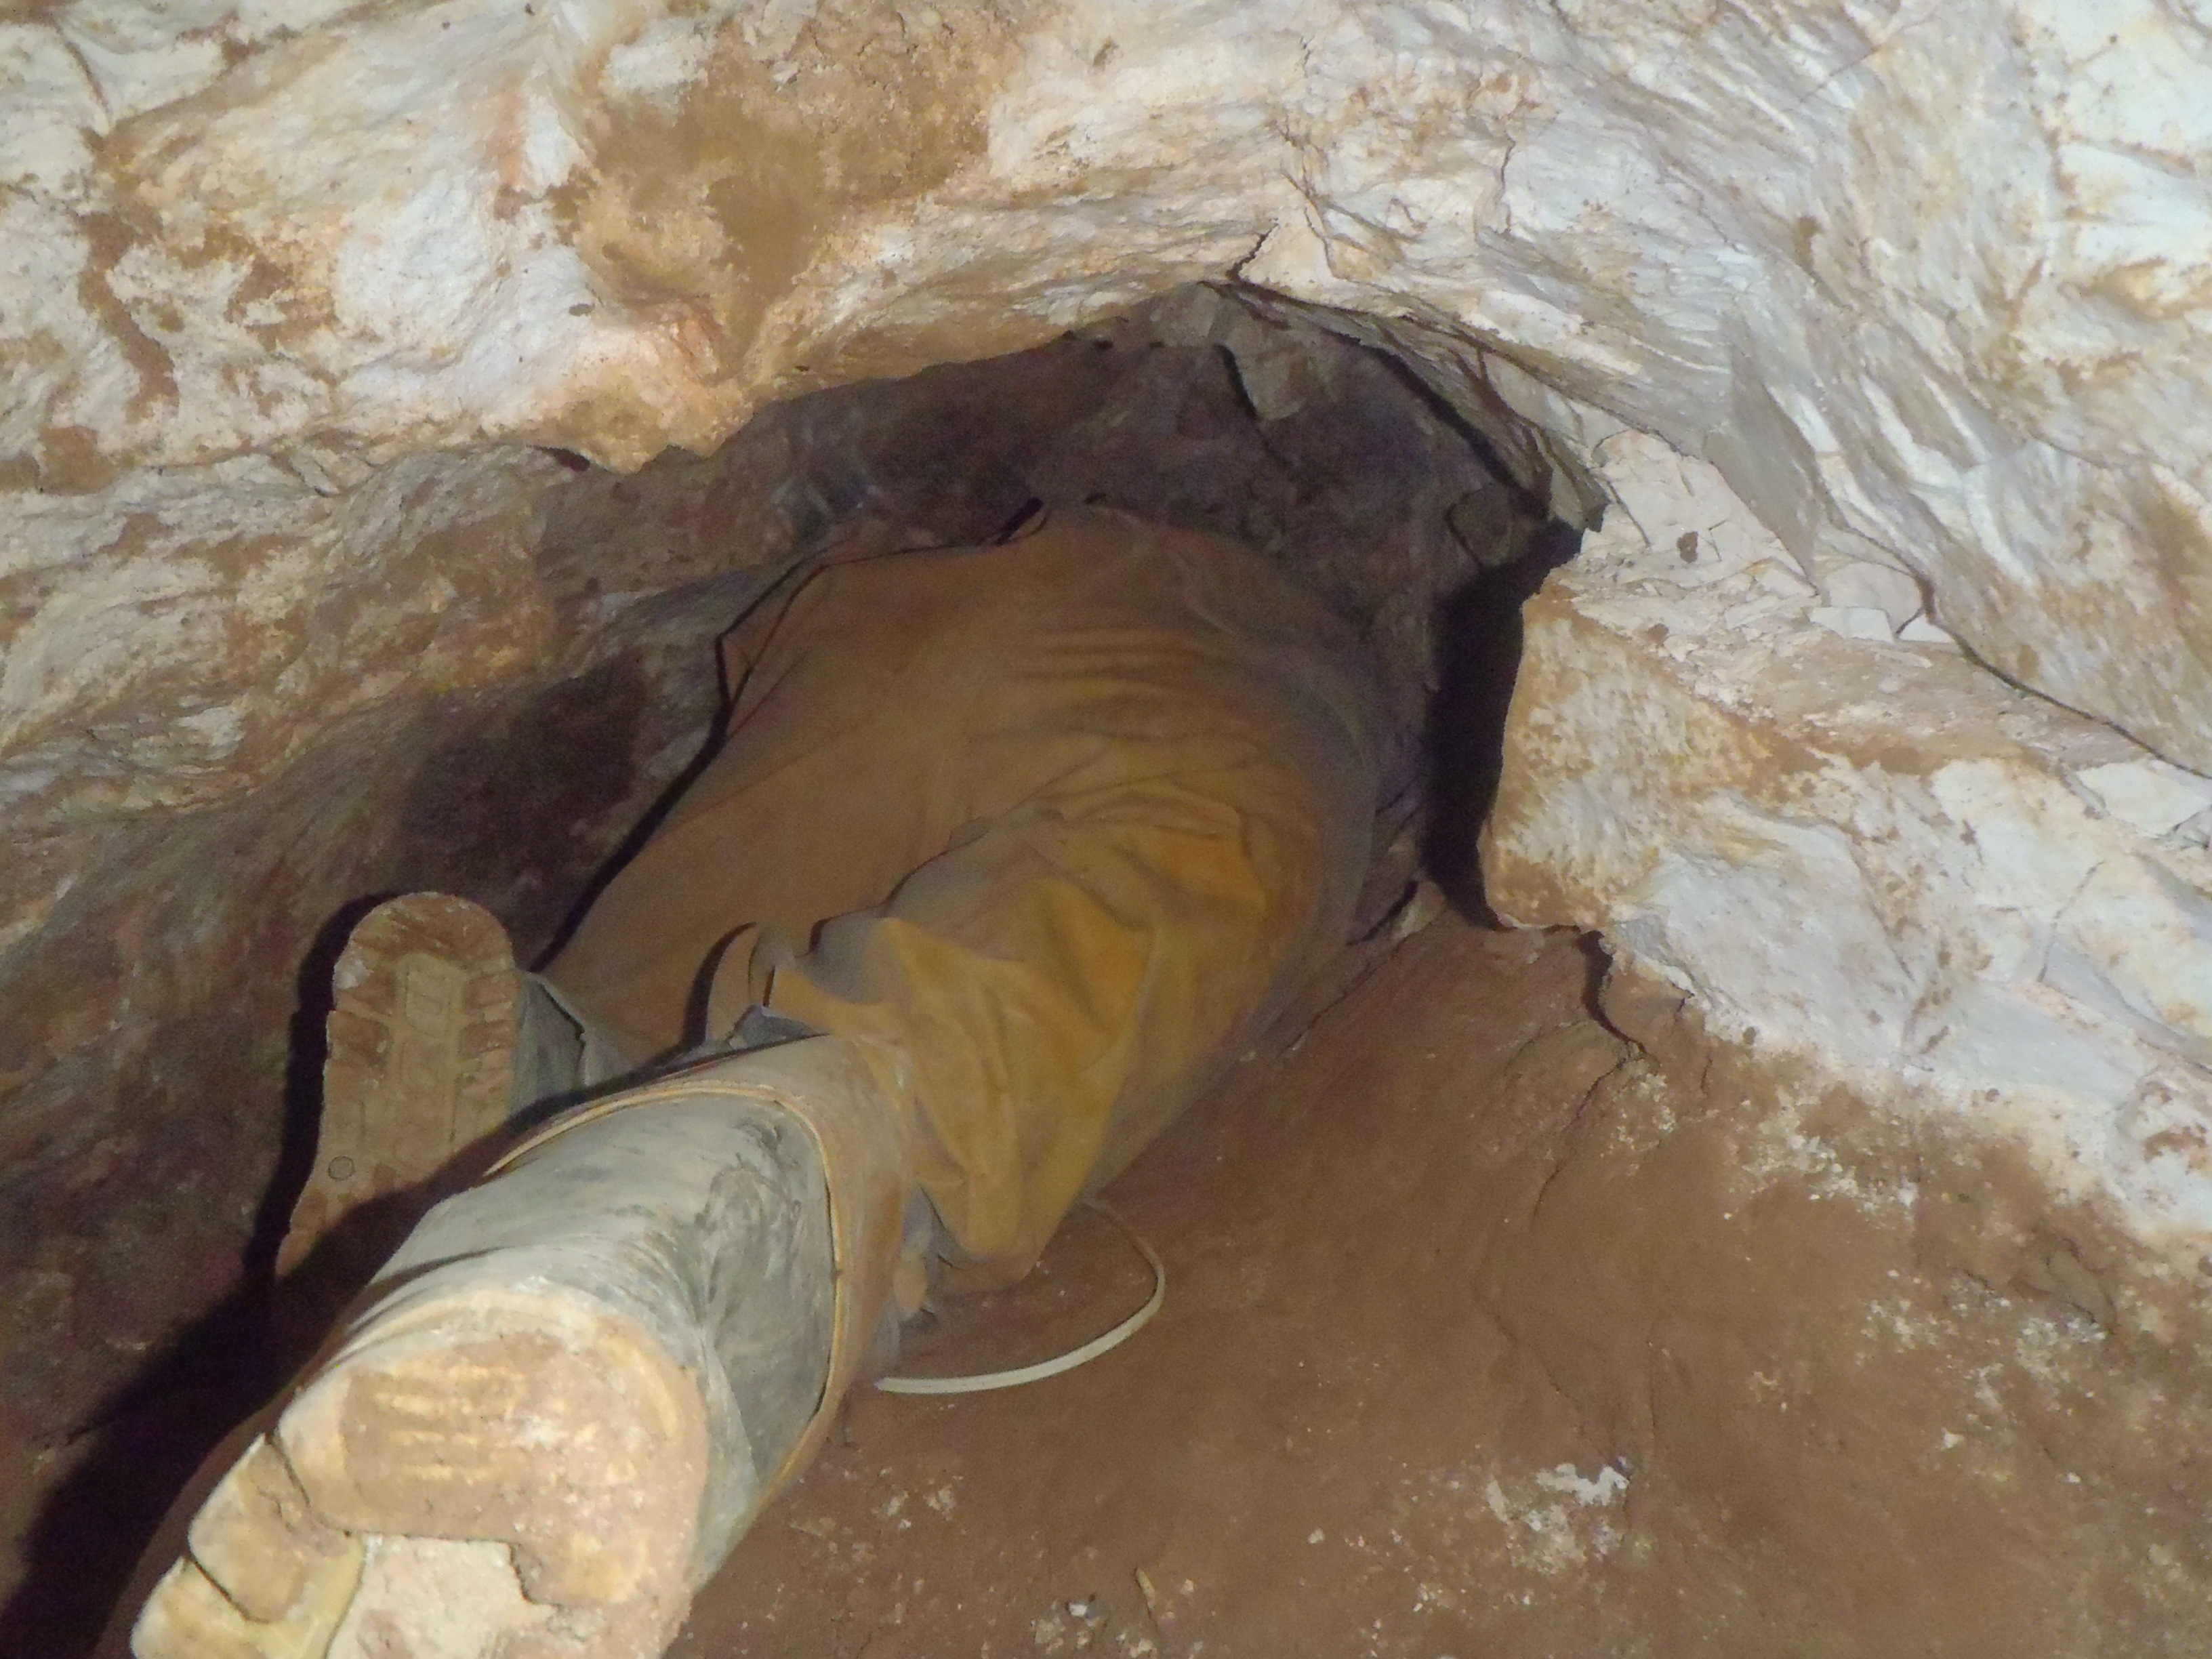
\includegraphics[width=\linewidth]{2012/discoveries/2012-07-31-1548-IztokMozir-P7310682--orig.jpg}} 
 \caption{Clare pushing the tight crawl in \passage{Wizard of Oz}. \pic{Iztok Možir}}
 \label{m2 crawl}
\end{marginfigure}

On the final attempt, the 8 m crawl in \passage{Wizard of Oz} was passed.
The passage enlarges into an immature rift but closes down almost
immediately with silt and mud flakes, without any sort of draught. About
midway through the crawl there seemed to be a very slight draught coming
from a small hole in the floor, though any pushing here would require
considerable effort spent digging.


\subsection{\passage{Watership
Down}}

\passage{Watership Down} is the continuation of \passage{Winter Journey}, a
system of abandoned bedding planes at -888 m in \passage{Vrtnarija}. Two
pushing trips were carried out to explore rabbit warren-like system of
crawls and chambers. From the \passage{Winter Journey} pushing front, a
series of steeply inclined bedding planes covered with a thick inch
layer of mud were passed to gain a beautiful, clear static sump.
Opposite the sump a passage leads off into a tight rift which was not
pushed to its end; it is most likely a dead inlet.

More interestingly, obvious traverses and windows above the sump were
gained to find another crawl which ended above yet another static sump.

There are still undropped pitches and windows to be looked at in
\passage{Watership Down}, though it is unlikely more depth will be added.

A total of 140.96 m of passage was found in \passage{Watership Down},
adding 12 m of depth to \passage{Vrtnarija}.


\begin{figure*}[t!]
\checkoddpage \ifoddpage \forcerectofloat \else \forceversofloat \fi
\frame{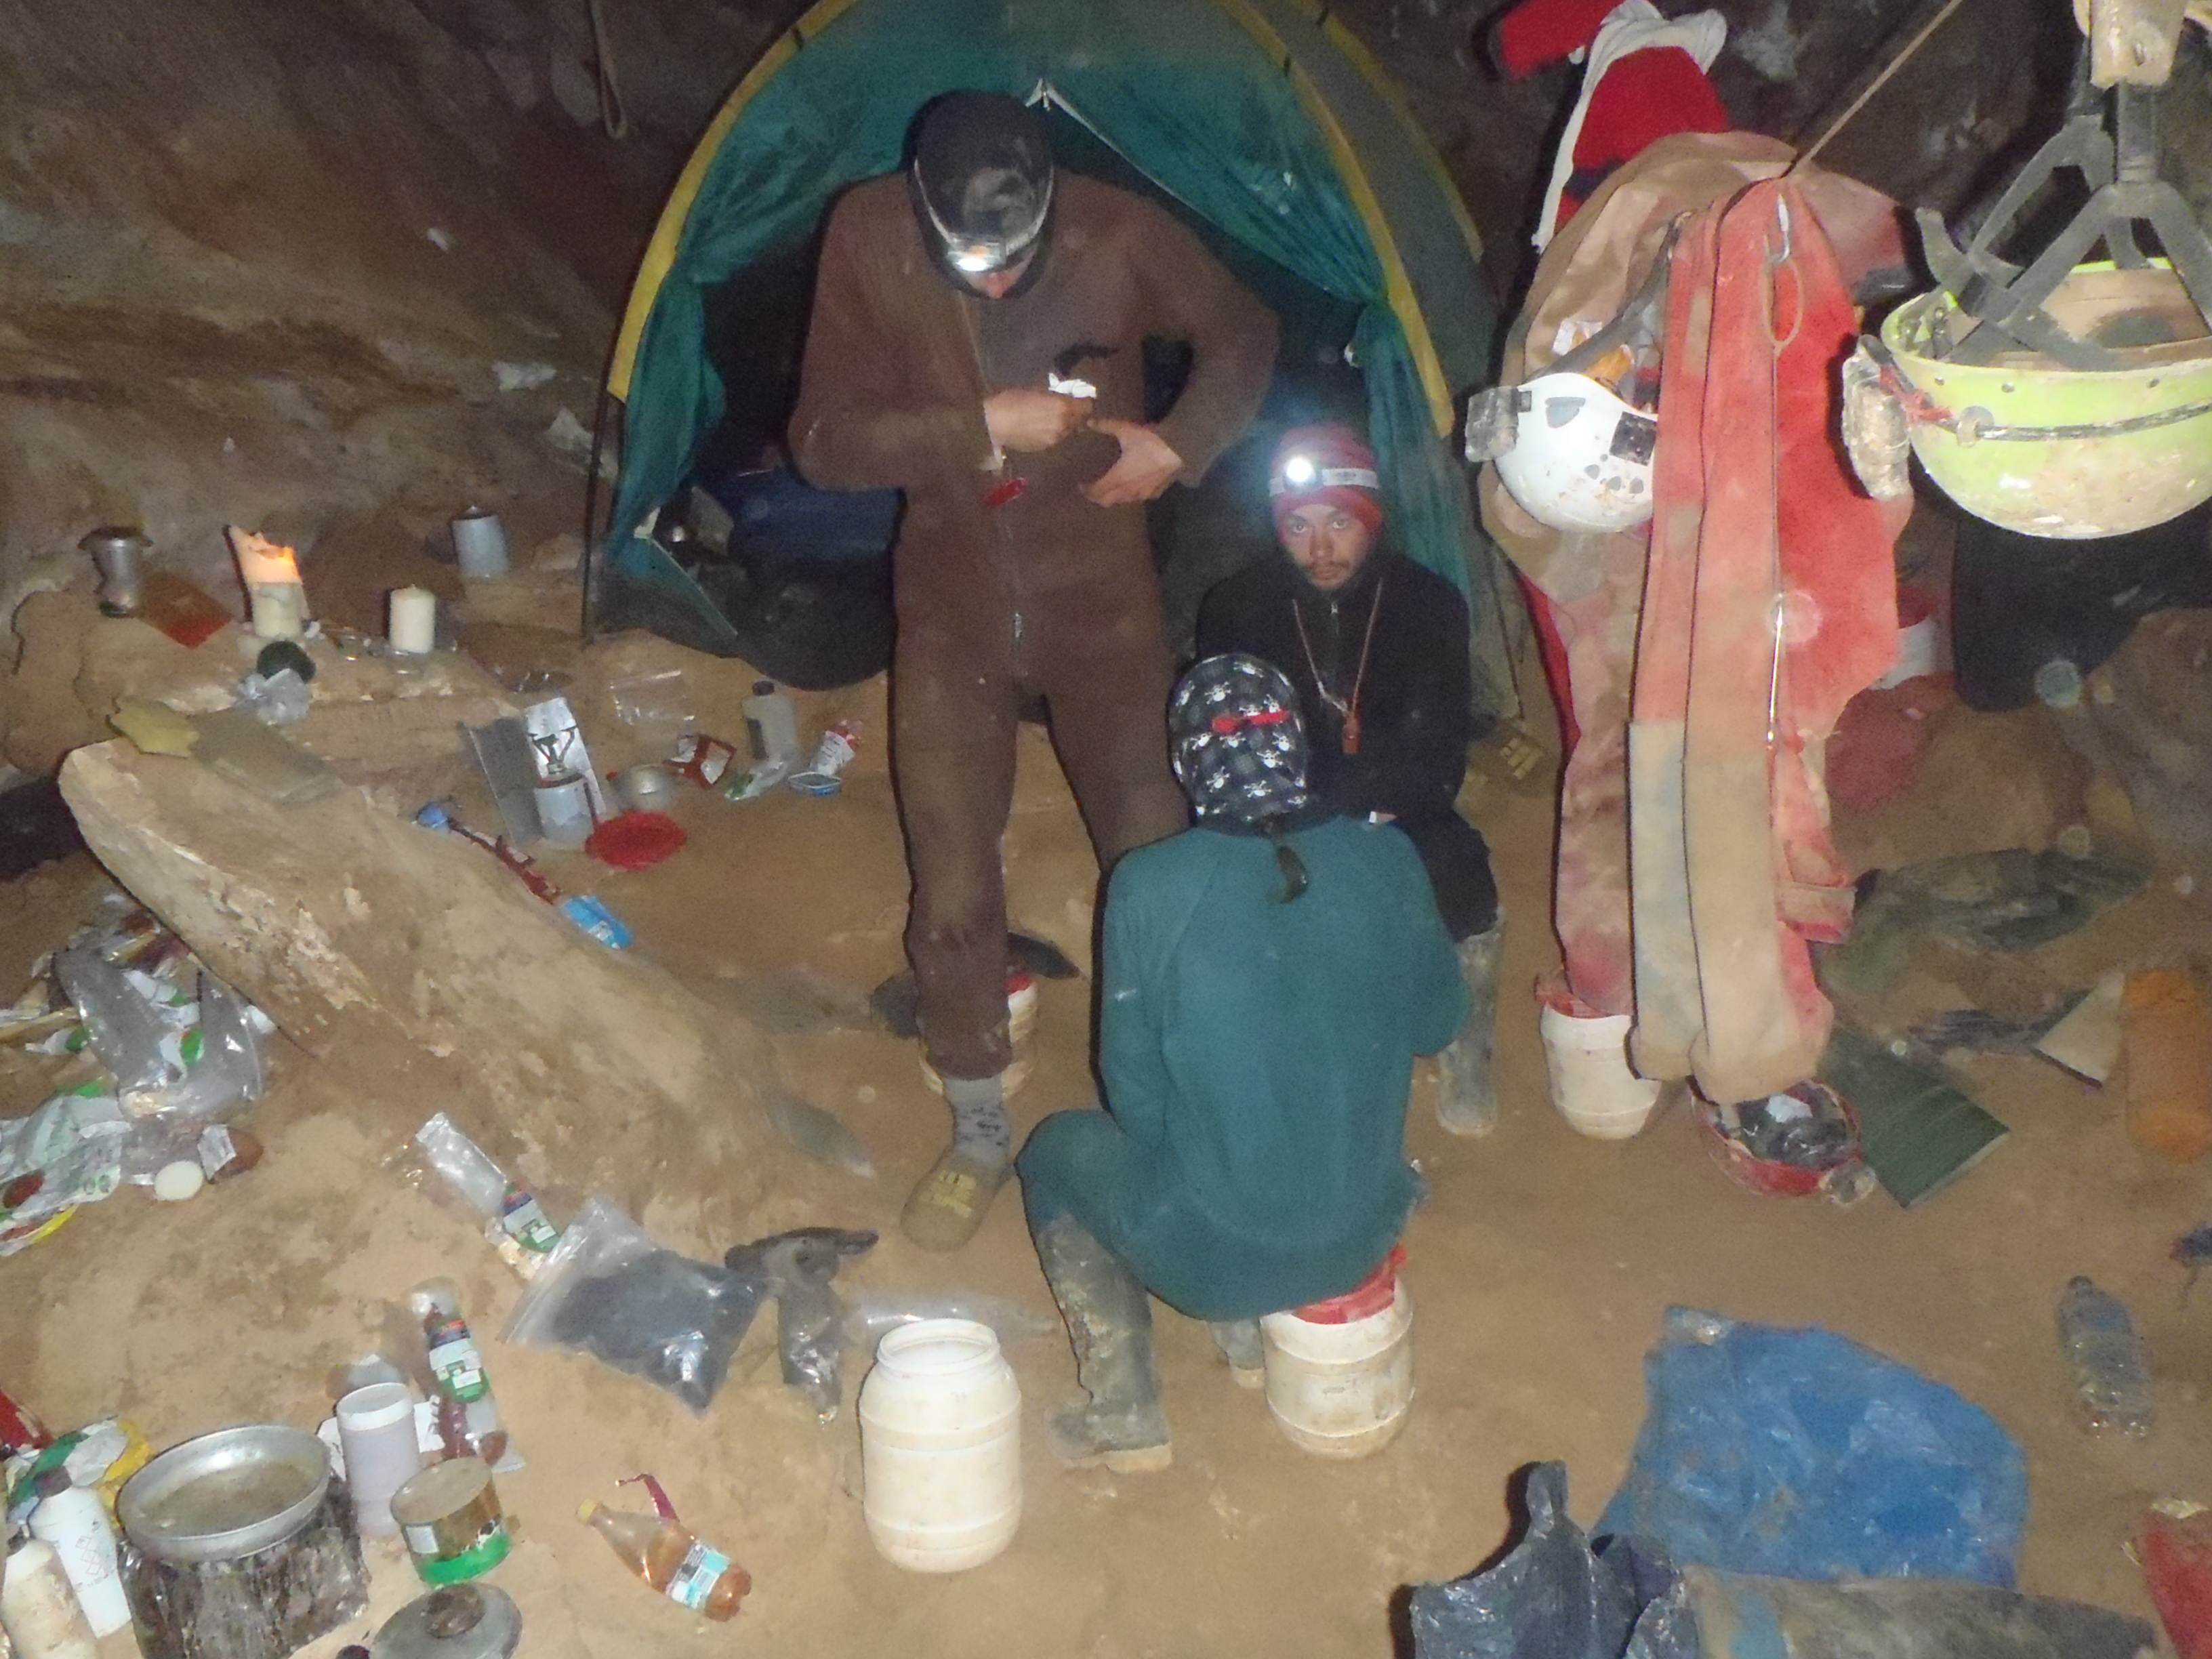
\includegraphics[width=\linewidth]{2012/discoveries/2012-08-04-0013-IztokMozir-P8040788--orig.jpg}}
\caption{Camp \protect\passage{X-Ray} was once again our base for exploring the depths of \passage{Vrtnarija}. \pic{Iztok Možir}} \label{x-ray 2012}
\end{figure*}



\subsection{Below `\passage{Stuck in
Paradise}'}

At the end of the 2011 expedition, \passage{Stuck in Paradise} (P69, -680
m) was dropped and two branches of extensive horizontal passage,
\passage{Salvation} and \passage{Lost Miles}, were found below it. The
possibility of more horizontal development at depth made the pushing of
\passage{Salvation} and \passage{Lost Miles} a high priority. \passage{Salvation}
The squeeze left at the end of \passage{Salvation} was hammered and dug
through to gain a small chamber with a roaring draught (\passage{Brave New
World}). The way on down was blocked by a big boulder choke; instead, a
carefully dug hole was followed upwards into sloping, crawling passage
that enlarges to walking height. Eventually, the passage breaks into an
active streamway, with the downstream passage taking the draught.

The downstream passage leads to an obvious phreatic continuation, which
was blocked by a collapsed ceiling. This boulder choke was eventually
squeezed through after two trips to reach 70 m of fine sandy passage
(\passage{Invictus}). This ends in a wet pitch ($\approx$ P20) that
was left unpushed.

172.4 m of mostly horizontal passage was found in the \passage{Salvation}
extensions.


\subsection{\passage{Lost
Miles}}

\begin{marginfigure}
\checkoddpage \ifoddpage \forcerectofloat \else \forceversofloat \fi
\centering
 \frame{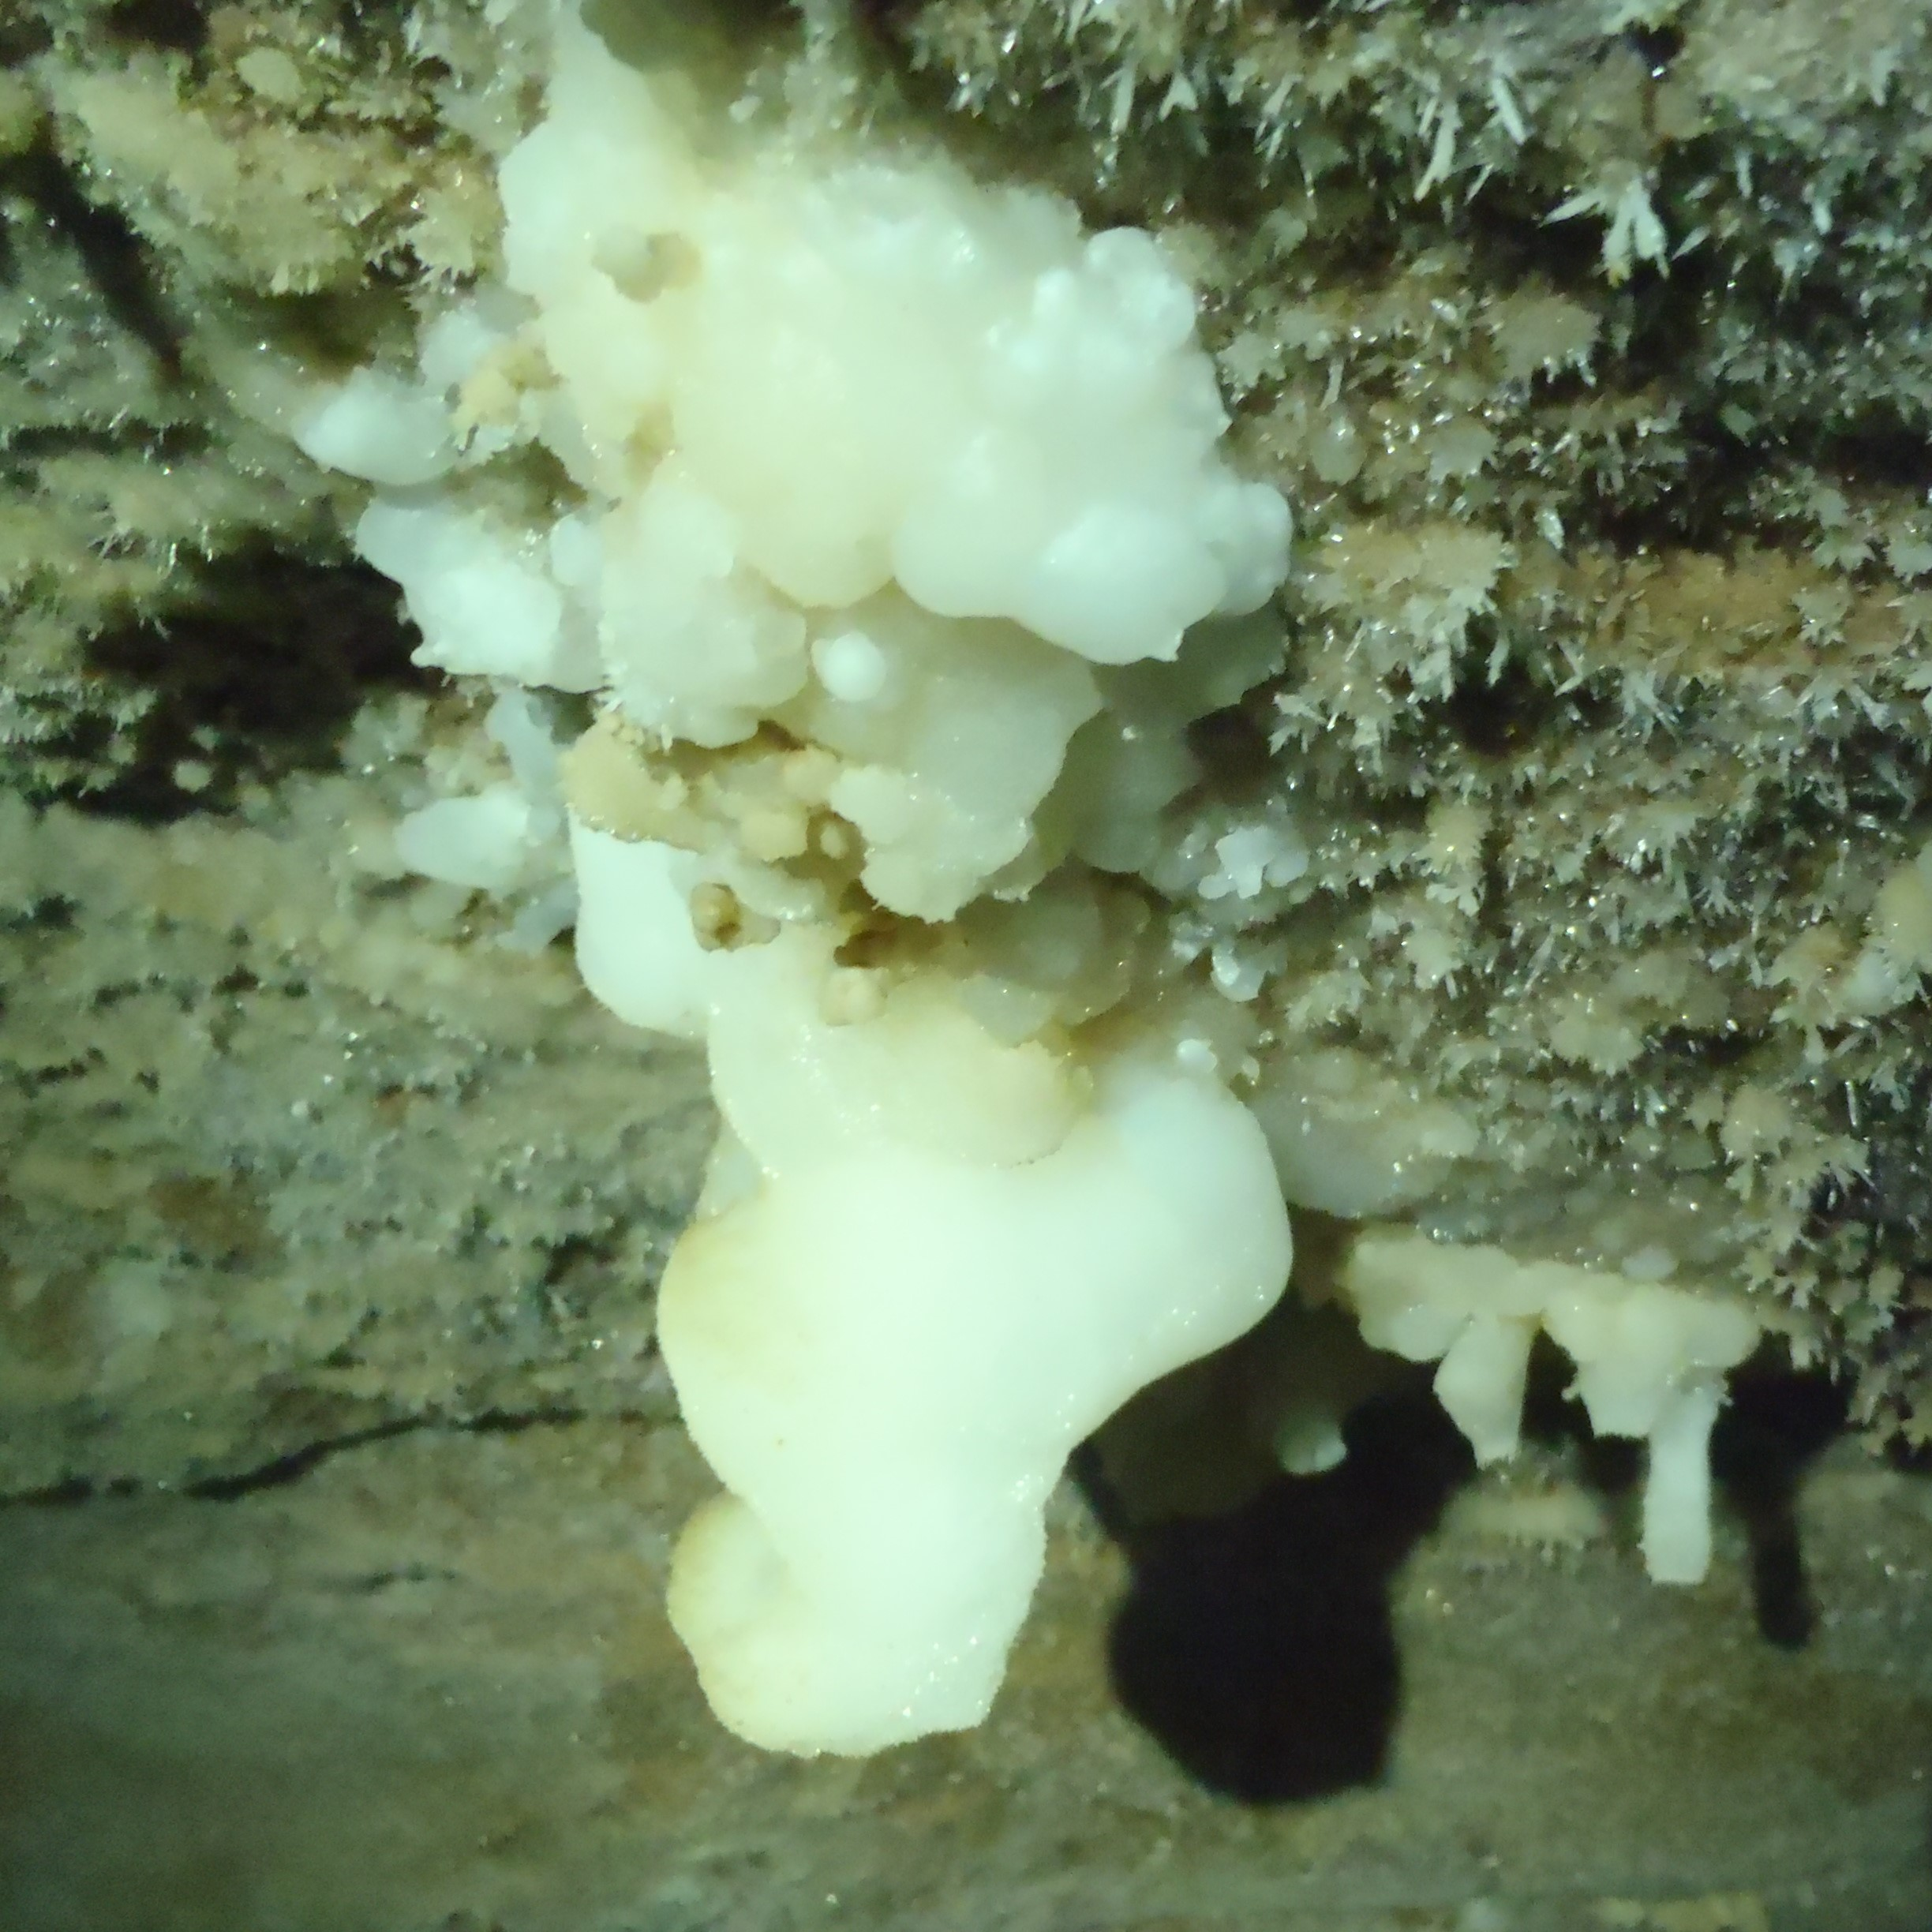
\includegraphics[width=\linewidth]{2012/discoveries/2012-08-03-0359-Maver-P8030152--orig.jpg}} 
 \caption{A formation and crystals in \passage{Brave New World}. \pic{Nejc Maver}}
 \label{bnw crystals}
\end{marginfigure}

At the end of the 2011 expedition, \passage{Lost Miles} was left as a
draughting boulder choke. This year, we managed to chisel and hammer our
way through, immediately breaking out into a large chamber and storming
passage (\passage{Atlantis}). After about 100 m a junction was reached with
three ways on: a pitch through a hole in the floor, a turning to the right, and continuation of the passage ahead.

The pitch was dropped, but leads almost immediately to a boulder choke
that looks promising but needs work (\passage{Inglourious Basterd}).

The passage on the right leads to about 250 m of easy caving, named \passage{Minestrone},
with occasional bouts of stooping and crawling. It eventually ends in a
small chamber, with the way on being a low crawl blocked by rubble,
though there is a draught. However, a subsequent digging trip to get
past the blockage was unsuccessful, and any further progress would
require considerable effort.

The continuation of \passage{Atlantis} led to more walking passage. Most
exciting was the discovery of a gallery of speleothems, including a vast
array of helictites, stalactites, stalagmites and columns. This is
probably the most decorated bit of cave we have found on \passage{Migovec} thus
far -- certainly the highest concentration of stal.

\begin{marginfigure}
\checkoddpage \ifoddpage \forcerectofloat \else \forceversofloat \fi
\centering
 \frame{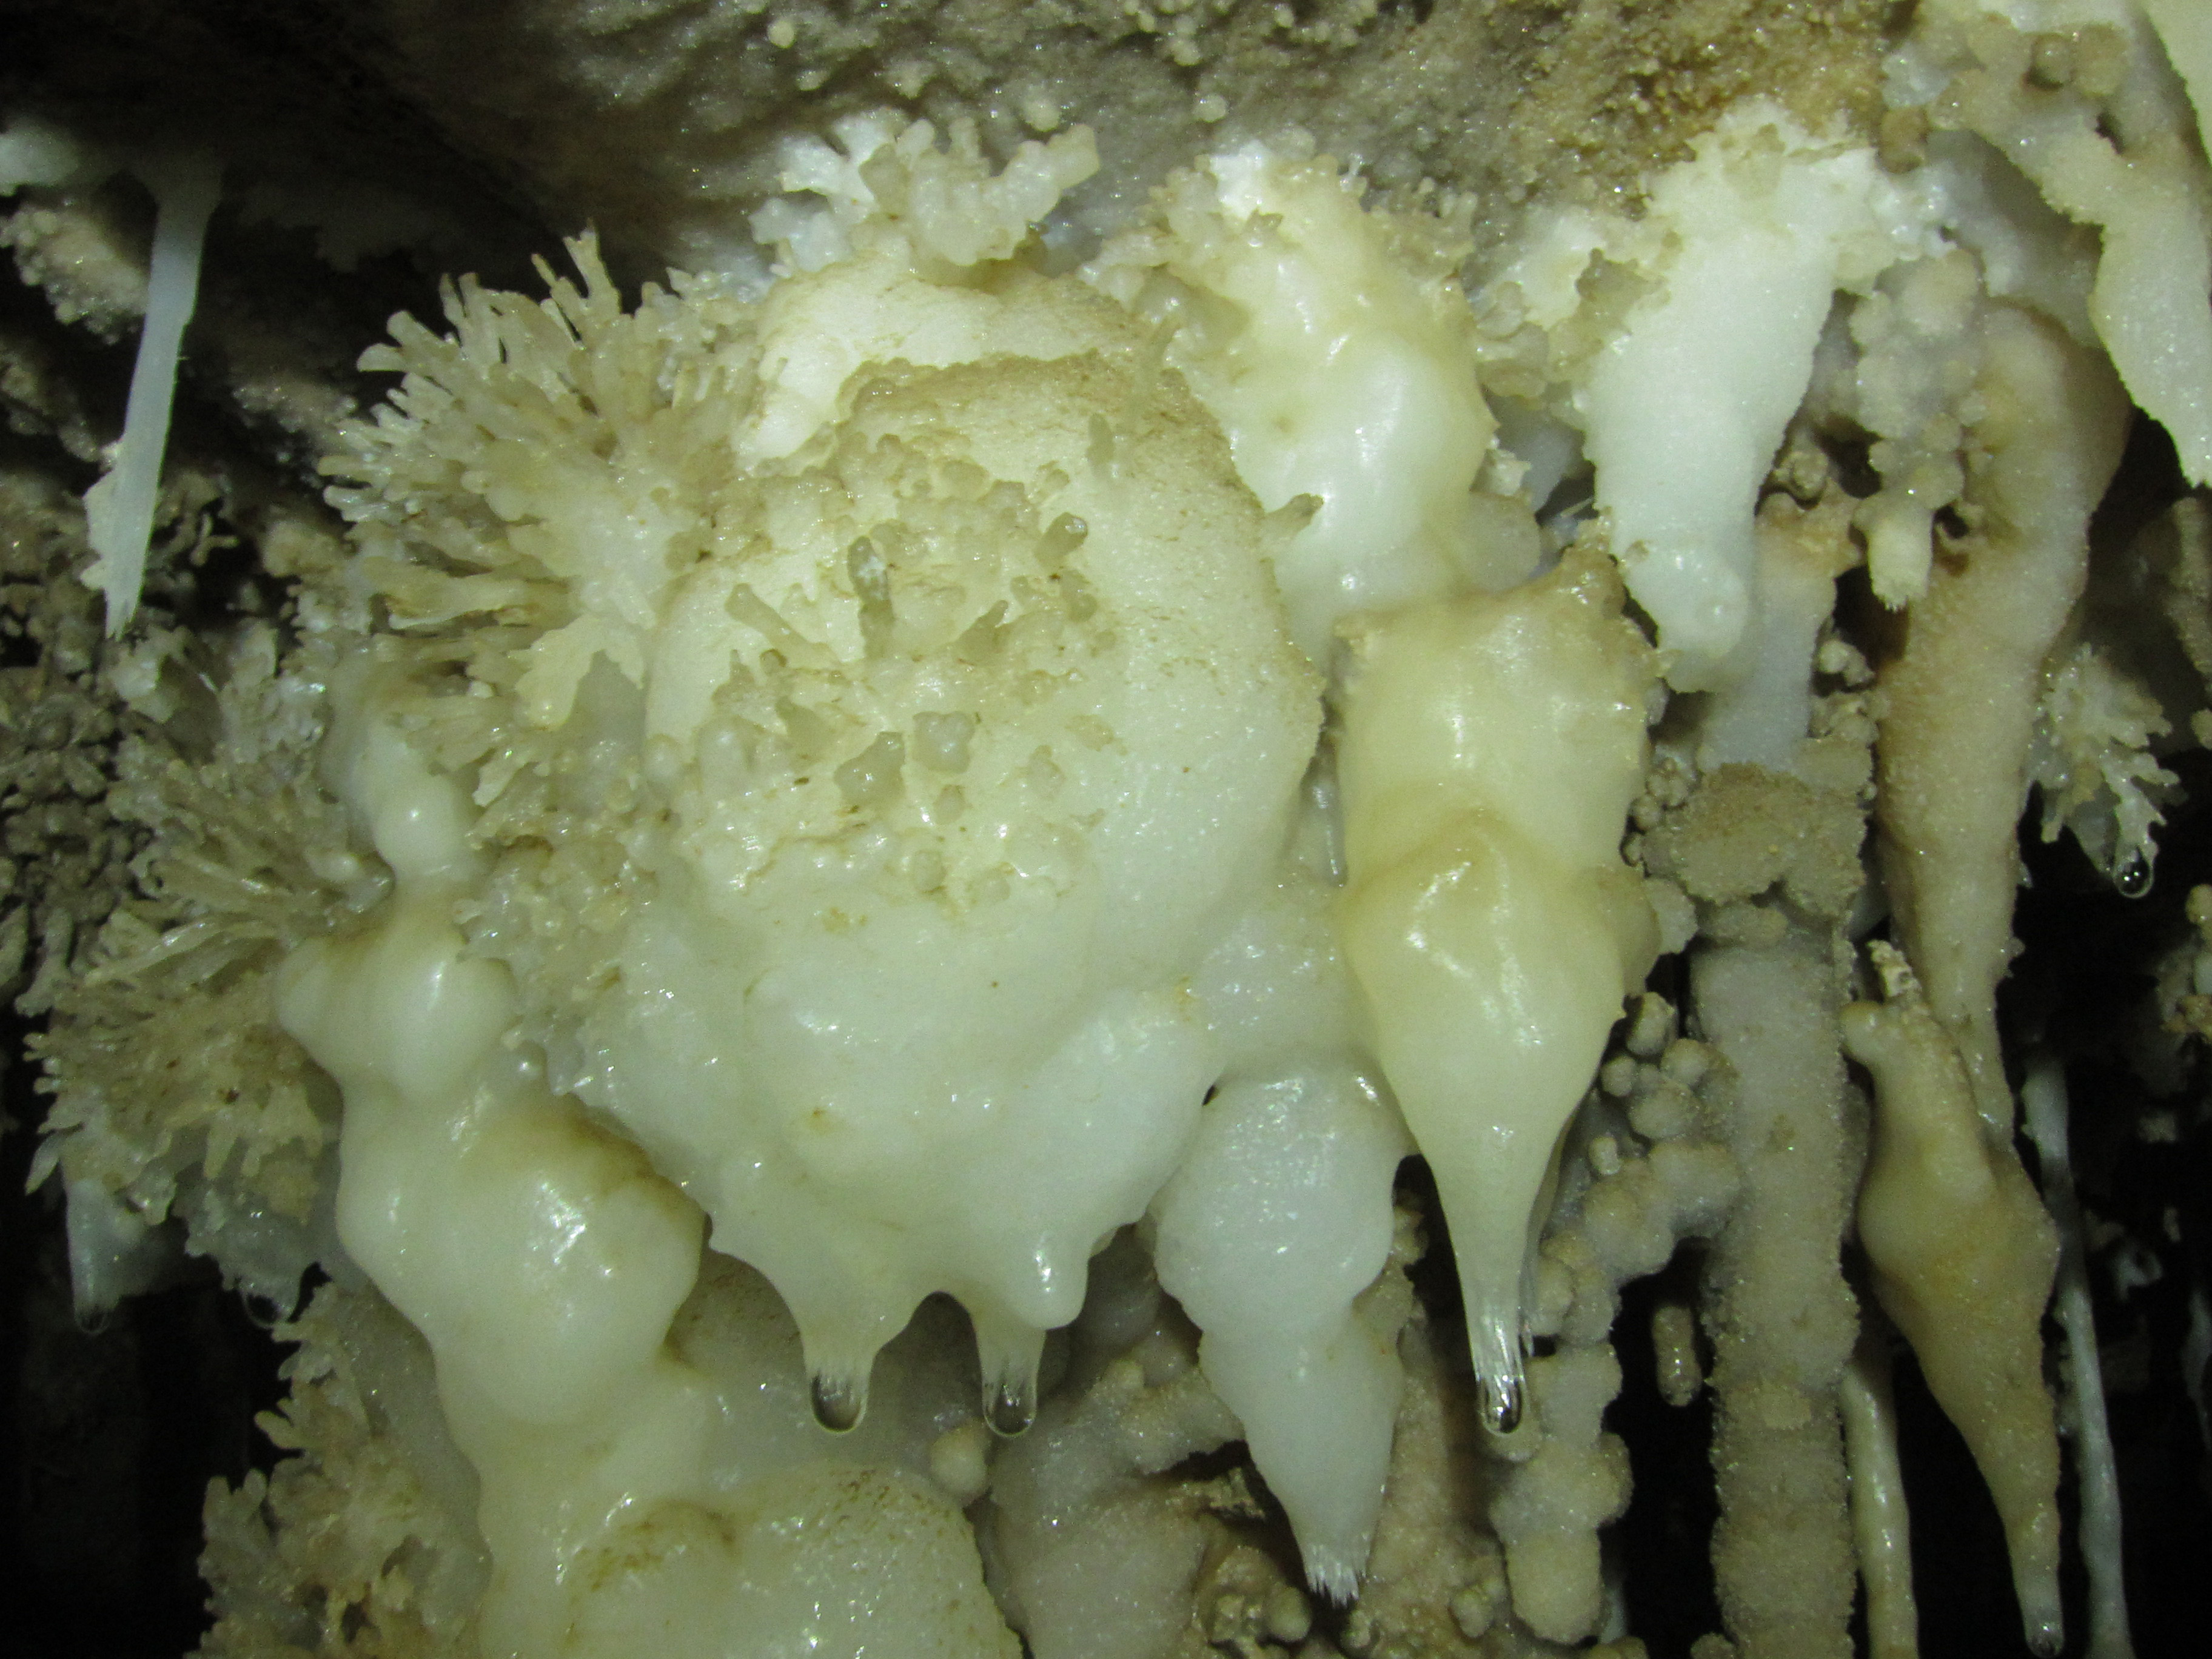
\includegraphics[width=\linewidth]{2012/discoveries/2012-08-03-0432-JanaCarga-028a--orig.jpg}} 
 \caption{Cave decorations in \passage{Atlantis}. \pic{Jana Carga}}
 \label{atlantis stal}
\end{marginfigure}


\passage{Atlantis} eventually becomes blocked with boulders in a low-roofed
passage. Straight on there is a tight squeeze through which the
continuation of the passage is visible. This was unpushed. Instead, a
squeeze under boulders on the right was passed to reach a small, dry
muddy tube that popped into a small chamber. The way on is a 10 m
flat-out crawl, accompanied by the sound of water. The crawl emerges in
a chamber at the bottom of a pitch, with a large waterfall entering from
above. This was thus named \passage{Brezno Slapov} (literally `waterfall
pitch').

A series of short cascades followed; exploration was eventually halted
by the need for rope.

A total of 757.15 m of passage was found beyond \passage{Lost Miles}.

Interestingly, these waterfall pitches found at the end of \passage{Brezno
Slapov} and \passage{Invictus} are the first signs of water and active
passage since \passage{Zimmer}.


\subsection{\passage{Apollo} \& the \passage{Milky
Way}}

In 2011, an attempt at a bolt climb to gain a window in the
\passage{Queen's Bedchamber} was derailed by bands of thick, slippery mud
preventing the successful installation of bolt belays. This year, armed
with tent pegs to hammer into the mud as temporary belays, three pushing
trips were required to conquer the bolt climb (\passage{Apollo}, P35).

At the top of the climb a muddy, downward-sloping passage leads to a
short pitch which lands in a large chamber. The passage on the right
leads to a dead end; the way on is through a short bedding crawl on the
left.

The crawl quickly widens into a small chamber with two ways on. Straight
ahead is easy but muddy caving, eventually leading to a pitch which we
suspect drops back into the \passage{Queen's Bedchamber}. On the right is a
long horizontal passage, mostly requiring easy crawling or stooping
(\passage{Milky Way}). At the end of this passage is a clean-washed chamber
that joins a split-pitch midway. A high, wet aven drops into the
chamber; the water then disappears under boulders. A way through the
boulder floor is obvious and easy, leading to a pitch. On a subsequent
trip this pitch was dropped but not surveyed.

Midway through \passage{Milky Way} is a turning off to the left, heading
south-west. This was pushed for about 70 m to a boulder choke that was
easily passed. Following the draught for about 50 m, a 20 m high rift
was eventually reached; this rift is most likely the continuation of the
\passage{Minotaur}/\passage{Guillotine} rift in \passage{Vrtnarija}.

From the rift, a horizontal, crystal-covered phreatic passage continues
South-West, heading directly towards \passage{System Migovec}. The phreatic seems
to have multiple levels, as it was sometimes possible to see empty space
between the boulders below.

A couple of climbs later, a $\approx$ 30 m wet pitch was reached.
A bigger dark space could be seen across the pitch, so a traverse line
was rigged. After 3 m of traversing, a bolt placed by cavers in 1998 was
found. Across the traverse lay a large chamber ($\approx$ 20 m
wide) in the middle of which a PSS was found: \passage{Waterloo}.13, dated
6/8/98, JE/IMcK (Jim Evans and Iain McKenna). On the last pushing day of the expedition, the
connection to \passage{System Migovec} was finally made! The passage was named
\passage{Dreams for the Soul}.

703.46 m of cave was found in the \passage{Apollo} extensions.


\subsection{The \passage{Throne
Room}}

At the end of 2011 expedition there were two unpushed leads in the
\passage{Throne Room}: a pitch, and a window across it. The pitch (\passage{Why the
face?}) was dropped. The crawl below it leads immediately to a draughting
pitch, which was also dropped but the passage below it quickly choked.

The traverse was bolted across to the window and up a steeply inclined,
very loose boulder slope (\passage{Hot Pants}). From the top of the traverse is a
short climb up the slope and through a boulder choke to a fairly
impressive chamber about 7 m high. A sandy tube goes from the edge of
the chamber, blowing out; it is fairly committing and was left unpushed
this expedition.

Two further trips were made to bolt climb up to the window in the
chamber and push the passage beyond. This climb reached a ledge in the
chamber, which gained parallel passage trending downwards at 30 degrees
and pushed for 70 m (\passage{Peep Show}).

Returning to the ledge, the upwards continuation (\passage{Undercover Squirrel})
was pushed for 70 m up a couple of free climbs. Exploration was halted
as a modest bolt climb was required to progress.

The area in general is of interest due to its location in the far
North-East of the known cave passage -- it is possible that it may access
more `deep level' galleries such as were discovered 300 m to the West
within the mountain in 2003 and 2004.

281.61 m of passage was found in the leads off The \passage{Throne Room}.


\subsection{\passage{Xanadu}}

\passage{Xanadu} is a new and exciting lead found in 2012. It starts from a
nondescript hole in the floor in \passage{Friendship Gallery}, a mere 5
minutes from Camp \passage{X-Ray} en route to \passage{Big Rock Candy
Mountain}. Surprisingly, no one explored it in the 9 years since we
first camped at \passage{X-Ray}!

The climb down through the hole immediately leads to an interesting rift
with different levels. At the bottom ($\approx$ 30 m below
\passage{Friendship Gallery}) is an active stream. Upstream was pushed to a
wet squeeze, downstream ended in a sump.

However, the most promising way on is midway down the rift, where it is
possible to gain a muddy, wet tube. Through this tube the character of
the cave changes completely, with dry, muddy passage (\passage{Euphrates}) instead
of the clean-washed white rock of before. At the end of the muddy
passage is a strongly draughting pitch.

Initial attempts to descend the pitch proved unsuccessful due to the
poor quality of rock. The pitch remains undescended and is an exciting
lead for 2013.

86.69 m was found in \passage{Xanadu}.


\subsection{\passage{Yorkshire}}

\passage{Yorkshire} is the continued exploration along a narrow rift above
an active waterfall at the bottom of the \passage{Lower Pleasures} series,
which was explored in 2011.

Initial narrow rift gives way to a squeeze above 2 m hole, which is
followed by another squeeze into a small chamber. Turning left from the
chamber quickly led to tight constriction from which an active stream
enters and exits to the right. Turning right led to more narrow rift,
which drops into a small pool of water after 8 m. A stream, which enters
the pool from the left, was followed downstream for another 30 m before
a dried mud junction was discovered at higher level.

The streamway continued further, but this was not surveyed.

The 2012 exploration of \passage{Yorkshire} found 91.18 m of passage, most
of which gently sloped northward, in parallel to \passage{Highway 32}, 35 m below.


\subsection{\passage{Minotaur
Rift}}

The squeeze left at the far end of \passage{Minotaur Rift} in the 2010
expedition was pushed to difficult crawling passage, often awkward with
loose, sharp rocks. The rift continues along the same fault line as in
\passage{Minotaur rift}. A series of boulder chokes make progress
interesting, including one which involves squeezing past a sharp rock,
precariously wedged above one's head (\passage{Guillotine}).

After \passage{Guillotine} is a very tight and sharp flat out crawl,
sloping slightly downwards. The passage eventually pops out into the
larger chamber. On inspection it proved to be a very big open fault
(\passage{Razor}). Looking up, a higher level can be observed. The way on
continues down a small pitch and a further two climbs down.
Unfortunately, the rift at the end gets too narrow to follow.

174.41 m was added to \passage{Minotaur Rift}.


\subsection{\passage{Stagger
Lee}}

In 2011, a window off the side of \passage{Big Rock Candy Mountain} was
spotted. \passage{Stagger Lee} is the continuation of this window located
17 m above the floor of \passage{Big Rock}. A high traverse was set up from the
second last hanger. It was followed by a 15 m abseil and another 5 m
traverse through falling water to gain the window.

Following the right hand side of the wall led to a series of cascading
drops (P35 m) that ended on the floor of the twin shaft. Here, two
streams combined into one active streamway beneath boulder-filled
chamber.

The streamway continued for a further 14 m before dropping 10 m into a
horizontal streamway which was later discovered to be the mouth of
\passage{Soda Stream}, killing interest in future exploration in this
chamber. Nonetheless a side window heading in the general direction of
\passage{Balamory} was spotted 4 m from the bottom.

A total of 145.01 m of passage was found in \passage{Stagger Lee}, part of
which was a resurvey of \passage{Soda Stream}.

\section{Surface Work}

“Surface bashing”, searching for new cave on the surface and investigating these new leads offers a welcome change to deep caving but is also essential for the life of the expedition. Efforts were made in both \passage{Area N} and \passage{Area K}.

\subsection{\passage{Area N}}

Arguably, the best new lead on the plateau is \passage{Kuk Pot} (\passage{N9}), discovered during a Winter Mountaineering search for blowing holes in December 2009. Two pitches were dropped in \passage{N9}, with the continuation visible but hampered by a lack of time. Unfortunately, \passage{Area N} is two hours walk from the Bivi, slowing the rate of exploration here.

\begin{figure}
\checkoddpage \ifoddpage \forcerectofloat \else \forceversofloat \fi
   \centering
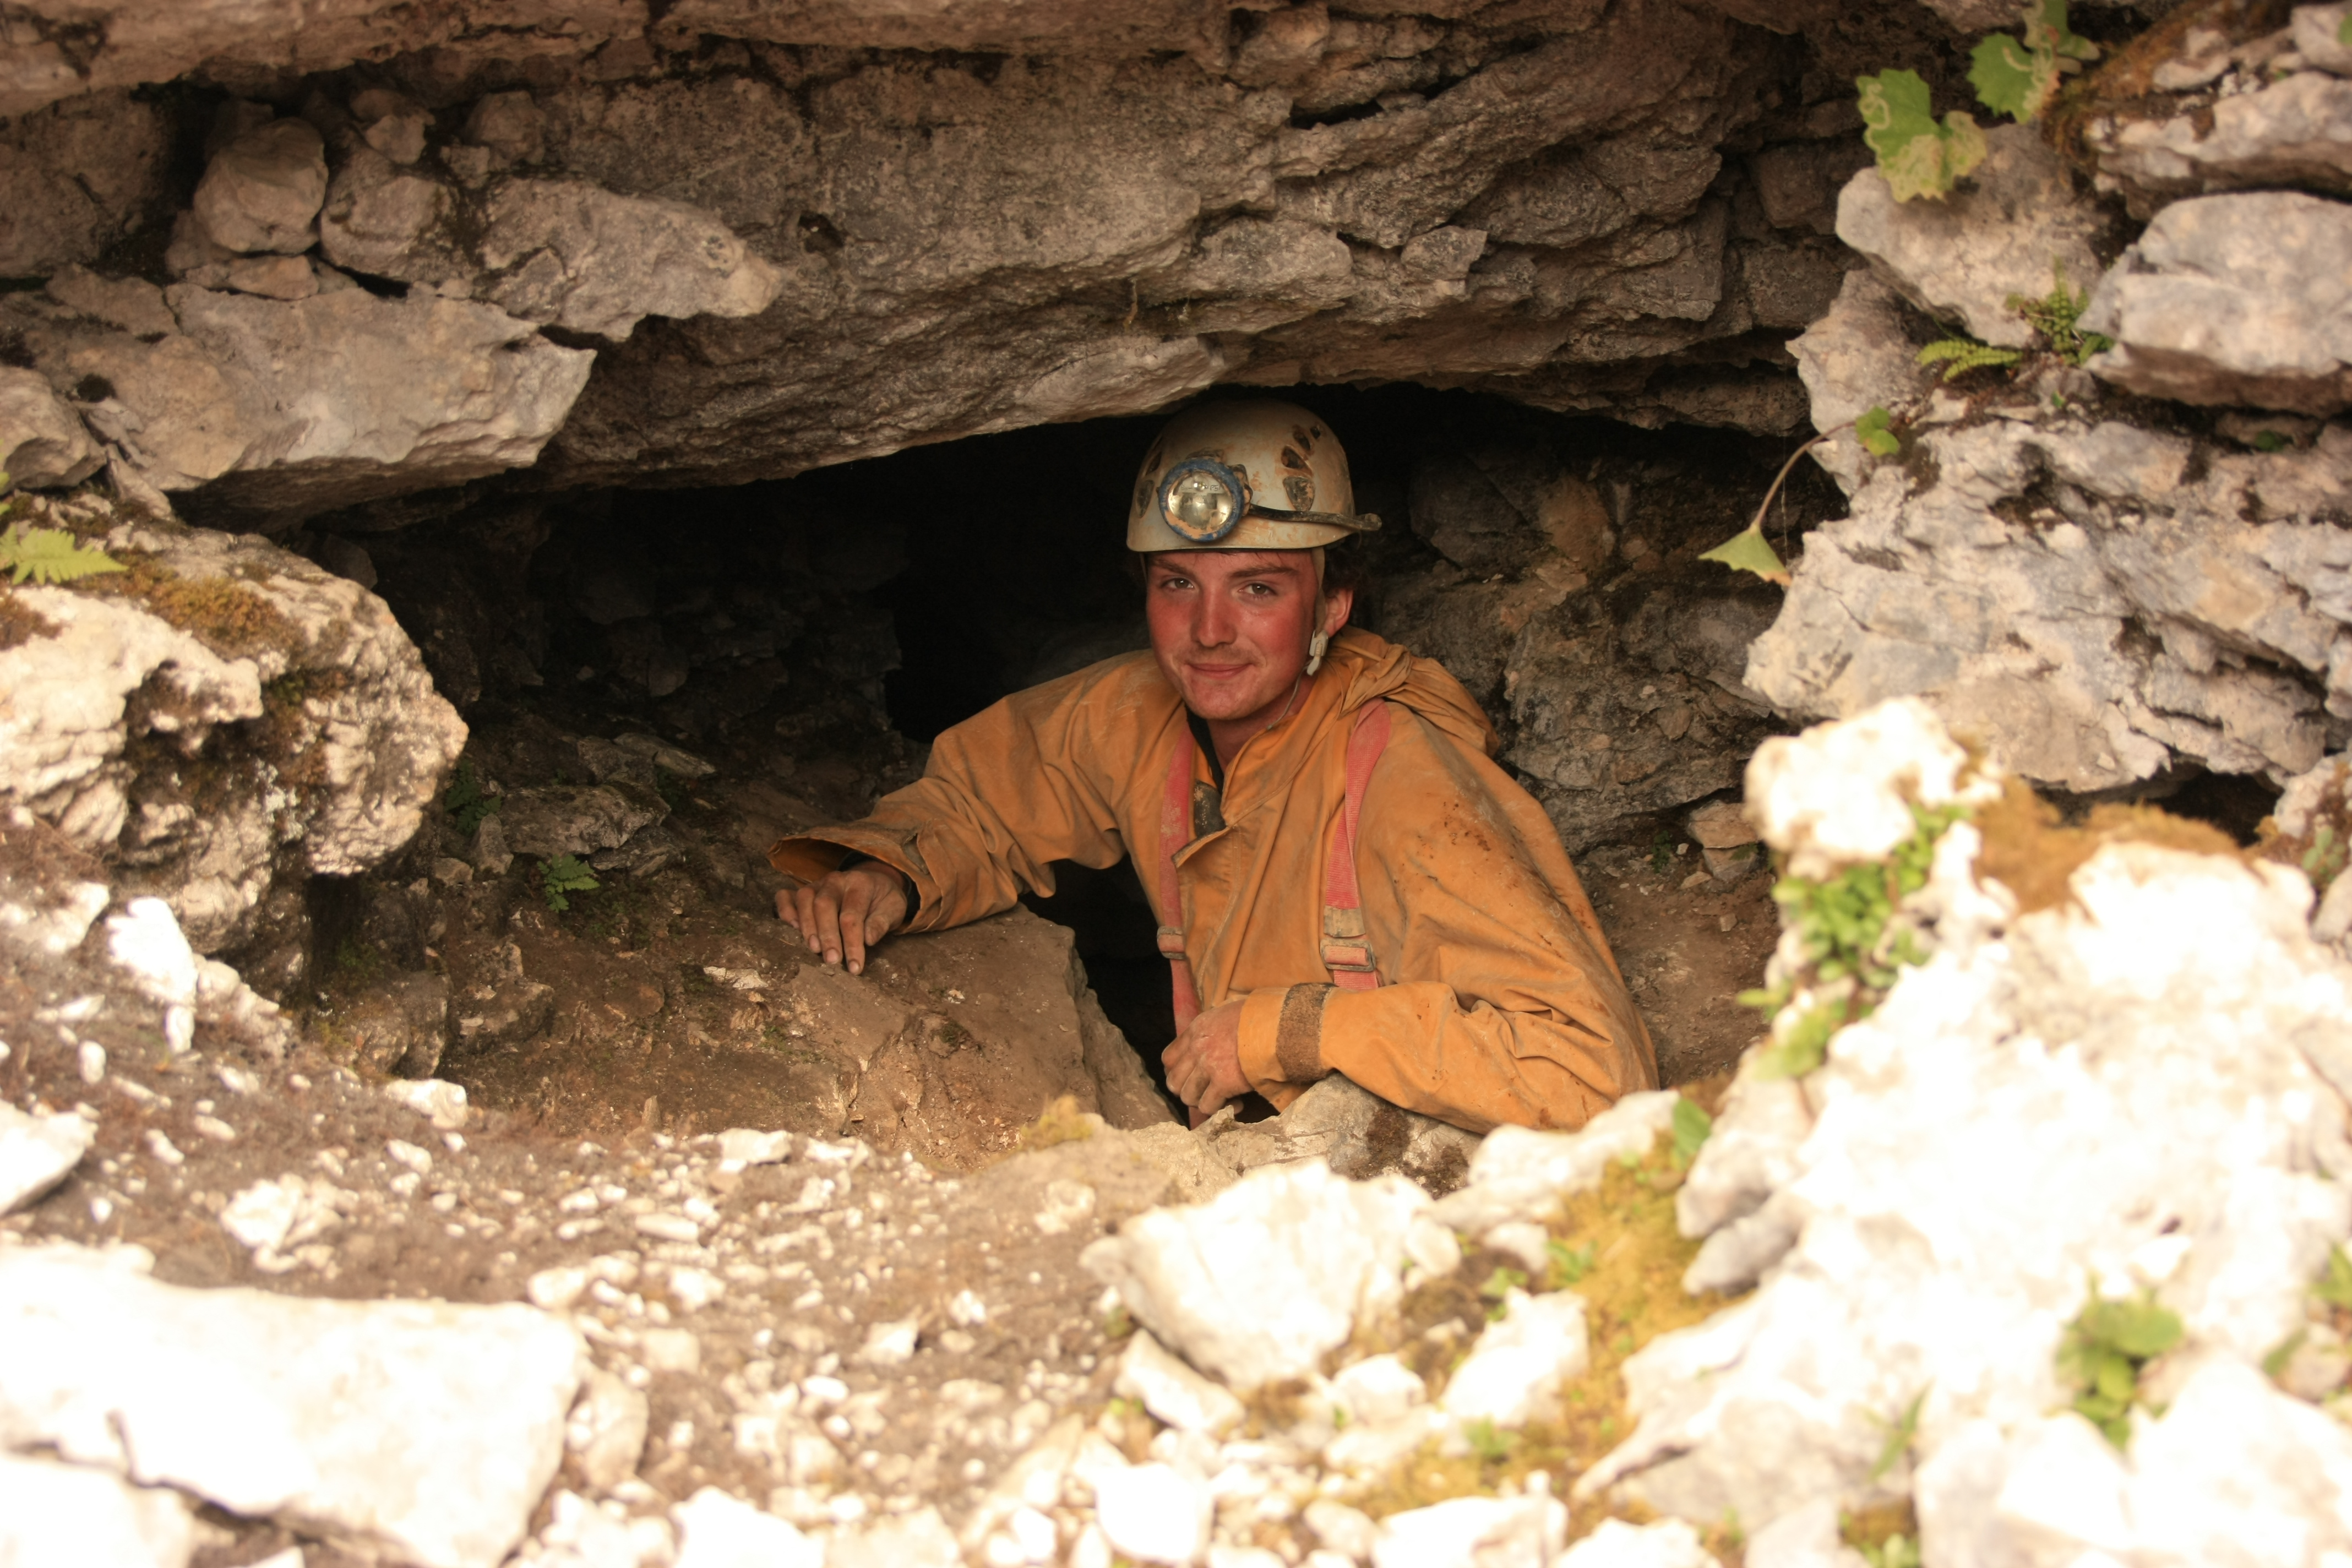
\includegraphics[width = \textwidth]{2012/discoveries/2012-08-10-0620-GergelyAmbrus-IMG_2275--N9--orig.jpg}
\caption{Jonny Hardman in the entrance of \passage{N9}. \pic{Gergely Ambrus}} \label{N9 entrance}
\end{figure}

\subsection{\passage{Area K}}

Area K is a valley to the north-east of the plateau, past the entrance to \passage{Vrtnarija} and just 30 minutes walk from the Bivi. Early in the expedition, one new cave was found and nine previously marked caves were re-evaluated: Entrances \passage{K2}, \passage{K6}, \passage{K11}, \passage{K22}, \passage{K21}, \passage{K23}, \passage{K24}, \passage{K25}, and \passage{K26}. \passage{K22}, \passage{K24}, \passage{K25} did not seem at all promising. 

Unfortunately, interest in these caves was concentrated into a relatively small group of cavers, who all left at the same time midway through the expedition. Some caves were dismissed (K2, “full of poo”) to the confusion of later visitors, although good progress was made digging at \passage{K6}. Of the remainder, \passage{K2} seems to have the most potential, though all need a lot of work before the cave goes.


\section{Super Action}

In October 2012, on the annual ICCC/JSPDT super action weekend, a
breakthrough was made in \passage{Primadona}, another cave system on
mountain. Due to its close proximity to the System, this will be the
next big connection project in our bid to shed more light on the complex
subterranean system under \passage{Migovec}.